\documentclass[twoside]{book}

% Packages required by doxygen
\usepackage{fixltx2e}
\usepackage{calc}
\usepackage{doxygen}
\usepackage[export]{adjustbox} % also loads graphicx
\usepackage{graphicx}
\usepackage[utf8]{inputenc}
\usepackage{makeidx}
\usepackage{multicol}
\usepackage{multirow}
\PassOptionsToPackage{warn}{textcomp}
\usepackage{textcomp}
\usepackage[nointegrals]{wasysym}
\usepackage[table]{xcolor}

% Font selection
\usepackage[T1]{fontenc}
\usepackage[scaled=.90]{helvet}
\usepackage{courier}
\usepackage{amssymb}
\usepackage{sectsty}
\renewcommand{\familydefault}{\sfdefault}
\allsectionsfont{%
  \fontseries{bc}\selectfont%
  \color{darkgray}%
}
\renewcommand{\DoxyLabelFont}{%
  \fontseries{bc}\selectfont%
  \color{darkgray}%
}
\newcommand{\+}{\discretionary{\mbox{\scriptsize$\hookleftarrow$}}{}{}}

% Page & text layout
\usepackage{geometry}
\geometry{%
  a4paper,%
  top=2.5cm,%
  bottom=2.5cm,%
  left=2.5cm,%
  right=2.5cm%
}
\tolerance=750
\hfuzz=15pt
\hbadness=750
\setlength{\emergencystretch}{15pt}
\setlength{\parindent}{0cm}
\setlength{\parskip}{3ex plus 2ex minus 2ex}
\makeatletter
\renewcommand{\paragraph}{%
  \@startsection{paragraph}{4}{0ex}{-1.0ex}{1.0ex}{%
    \normalfont\normalsize\bfseries\SS@parafont%
  }%
}
\renewcommand{\subparagraph}{%
  \@startsection{subparagraph}{5}{0ex}{-1.0ex}{1.0ex}{%
    \normalfont\normalsize\bfseries\SS@subparafont%
  }%
}
\makeatother

% Headers & footers
\usepackage{fancyhdr}
\pagestyle{fancyplain}
\fancyhead[LE]{\fancyplain{}{\bfseries\thepage}}
\fancyhead[CE]{\fancyplain{}{}}
\fancyhead[RE]{\fancyplain{}{\bfseries\leftmark}}
\fancyhead[LO]{\fancyplain{}{\bfseries\rightmark}}
\fancyhead[CO]{\fancyplain{}{}}
\fancyhead[RO]{\fancyplain{}{\bfseries\thepage}}
\fancyfoot[LE]{\fancyplain{}{}}
\fancyfoot[CE]{\fancyplain{}{}}
\fancyfoot[RE]{\fancyplain{}{\bfseries\scriptsize Generated by Doxygen }}
\fancyfoot[LO]{\fancyplain{}{\bfseries\scriptsize Generated by Doxygen }}
\fancyfoot[CO]{\fancyplain{}{}}
\fancyfoot[RO]{\fancyplain{}{}}
\renewcommand{\footrulewidth}{0.4pt}
\renewcommand{\chaptermark}[1]{%
  \markboth{#1}{}%
}
\renewcommand{\sectionmark}[1]{%
  \markright{\thesection\ #1}%
}

% Indices & bibliography
\usepackage{natbib}
\usepackage[titles]{tocloft}
\setcounter{tocdepth}{3}
\setcounter{secnumdepth}{5}
\makeindex

% Hyperlinks (required, but should be loaded last)
\usepackage{ifpdf}
\ifpdf
  \usepackage[pdftex,pagebackref=true]{hyperref}
\else
  \usepackage[ps2pdf,pagebackref=true]{hyperref}
\fi
\hypersetup{%
  colorlinks=true,%
  linkcolor=blue,%
  citecolor=blue,%
  unicode%
}

% Custom commands
\newcommand{\clearemptydoublepage}{%
  \newpage{\pagestyle{empty}\cleardoublepage}%
}

\usepackage{caption}
\captionsetup{labelsep=space,justification=centering,font={bf},singlelinecheck=off,skip=4pt,position=top}

%===== C O N T E N T S =====

\begin{document}

% Titlepage & ToC
\hypersetup{pageanchor=false,
             bookmarksnumbered=true,
             pdfencoding=unicode
            }
\pagenumbering{alph}
\begin{titlepage}
\vspace*{7cm}
\begin{center}%
{\Large Projeto classes abstratas \\[1ex]\large 1.\+1 }\\
\vspace*{1cm}
{\large Generated by Doxygen 1.8.14}\\
\end{center}
\end{titlepage}
\clearemptydoublepage
\pagenumbering{roman}
\tableofcontents
\clearemptydoublepage
\pagenumbering{arabic}
\hypersetup{pageanchor=true}

%--- Begin generated contents ---
\chapter{Hierarchical Index}
\section{Class Hierarchy}
This inheritance list is sorted roughly, but not completely, alphabetically\+:\begin{DoxyCompactList}
\item \contentsline{section}{Data\+Storage}{\pageref{class_data_storage}}{}
\item \contentsline{section}{Entry}{\pageref{struct_entry}}{}
\item Q\+Main\+Window\begin{DoxyCompactList}
\item \contentsline{section}{Main\+Window}{\pageref{class_main_window}}{}
\end{DoxyCompactList}
\item \contentsline{section}{qt\+\_\+meta\+\_\+stringdata\+\_\+\+Main\+Window\+\_\+t}{\pageref{structqt__meta__stringdata___main_window__t}}{}
\item \contentsline{section}{qt\+\_\+meta\+\_\+stringdata\+\_\+\+My\+Server\+\_\+t}{\pageref{structqt__meta__stringdata___my_server__t}}{}
\item \contentsline{section}{qt\+\_\+meta\+\_\+stringdata\+\_\+\+My\+Thread\+\_\+t}{\pageref{structqt__meta__stringdata___my_thread__t}}{}
\item Q\+Tcp\+Server\begin{DoxyCompactList}
\item \contentsline{section}{My\+Server}{\pageref{class_my_server}}{}
\end{DoxyCompactList}
\item Q\+Thread\begin{DoxyCompactList}
\item \contentsline{section}{My\+Thread}{\pageref{class_my_thread}}{}
\end{DoxyCompactList}
\item \contentsline{section}{Range\+Test}{\pageref{struct_range_test}}{}
\item \contentsline{section}{Ui\+\_\+\+Main\+Window}{\pageref{class_ui___main_window}}{}
\begin{DoxyCompactList}
\item \contentsline{section}{Ui\+:\+:Main\+Window}{\pageref{class_ui_1_1_main_window}}{}
\end{DoxyCompactList}
\end{DoxyCompactList}

\chapter{Class Index}
\section{Class List}
Here are the classes, structs, unions and interfaces with brief descriptions\+:\begin{DoxyCompactList}
\item\contentsline{section}{\mbox{\hyperlink{class_main_window}{Main\+Window}} \\*The \mbox{\hyperlink{class_main_window}{Main\+Window}} class Classe da janela principal do consumidor de dados }{\pageref{class_main_window}}{}
\item\contentsline{section}{\mbox{\hyperlink{classplotter}{plotter}} \\*The plotter class Classe responsável por representar um gráfico através de um widget }{\pageref{classplotter}}{}
\end{DoxyCompactList}

\chapter{File Index}
\section{File List}
Here is a list of all files with brief descriptions\+:\begin{DoxyCompactList}
\item\contentsline{section}{\mbox{\hyperlink{main_8cpp}{main.\+cpp}} }{\pageref{main_8cpp}}{}
\item\contentsline{section}{\mbox{\hyperlink{mainwindow_8cpp}{mainwindow.\+cpp}} }{\pageref{mainwindow_8cpp}}{}
\item\contentsline{section}{\mbox{\hyperlink{mainwindow_8h}{mainwindow.\+h}} }{\pageref{mainwindow_8h}}{}
\end{DoxyCompactList}

\chapter{Class Documentation}
\hypertarget{class_circulo}{}\section{Circulo Class Reference}
\label{class_circulo}\index{Circulo@{Circulo}}


The \mbox{\hyperlink{class_circulo}{Circulo}} class Classe para representar uma circunferência ou disco.  




{\ttfamily \#include $<$circulo.\+h$>$}

Inheritance diagram for Circulo\+:\begin{figure}[H]
\begin{center}
\leavevmode
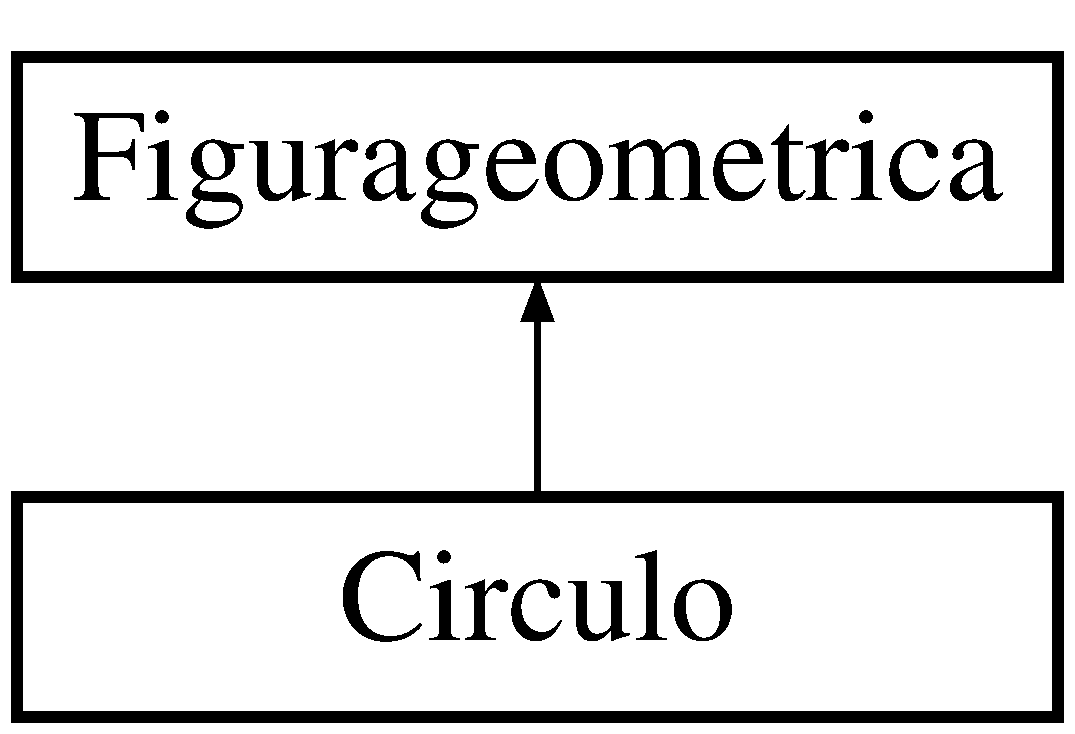
\includegraphics[height=2.000000cm]{class_circulo}
\end{center}
\end{figure}
\subsection*{Public Member Functions}
\begin{DoxyCompactItemize}
\item 
\mbox{\hyperlink{class_circulo_a0773937be6980f57837cb406d7553df8}{Circulo}} (\mbox{\hyperlink{class_ponto}{Ponto}} p1, int \+\_\+raio, bool \+\_\+fillmolde)
\begin{DoxyCompactList}\small\item\em \mbox{\hyperlink{class_circulo}{Circulo}} Construtor da classe circulo com parâmetros iniciais. \end{DoxyCompactList}\item 
void \mbox{\hyperlink{class_circulo_a593787d6e0618c2eded23e8839e7bea6}{draw}} (\mbox{\hyperlink{class_screen}{Screen}} \&t)
\begin{DoxyCompactList}\small\item\em draw Função virtual da classe circulo \end{DoxyCompactList}\end{DoxyCompactItemize}
\subsection*{Additional Inherited Members}


\subsection{Detailed Description}
The \mbox{\hyperlink{class_circulo}{Circulo}} class Classe para representar uma circunferência ou disco. 

\subsection{Constructor \& Destructor Documentation}
\mbox{\Hypertarget{class_circulo_a0773937be6980f57837cb406d7553df8}\label{class_circulo_a0773937be6980f57837cb406d7553df8}} 
\index{Circulo@{Circulo}!Circulo@{Circulo}}
\index{Circulo@{Circulo}!Circulo@{Circulo}}
\subsubsection{\texorpdfstring{Circulo()}{Circulo()}}
{\footnotesize\ttfamily Circulo\+::\+Circulo (\begin{DoxyParamCaption}\item[{\mbox{\hyperlink{class_ponto}{Ponto}}}]{p1,  }\item[{int}]{\+\_\+raio,  }\item[{bool}]{\+\_\+fillmolde }\end{DoxyParamCaption})}



\mbox{\hyperlink{class_circulo}{Circulo}} Construtor da classe circulo com parâmetros iniciais. 


\begin{DoxyParams}{Parameters}
{\em p1} & Coordenada do centro do circulo \\
\hline
{\em \+\_\+raio} & Raio do circulo \\
\hline
{\em \+\_\+fillmolde} & Variável que indica o modo de impressão \\
\hline
\end{DoxyParams}


\subsection{Member Function Documentation}
\mbox{\Hypertarget{class_circulo_a593787d6e0618c2eded23e8839e7bea6}\label{class_circulo_a593787d6e0618c2eded23e8839e7bea6}} 
\index{Circulo@{Circulo}!draw@{draw}}
\index{draw@{draw}!Circulo@{Circulo}}
\subsubsection{\texorpdfstring{draw()}{draw()}}
{\footnotesize\ttfamily void Circulo\+::draw (\begin{DoxyParamCaption}\item[{\mbox{\hyperlink{class_screen}{Screen}} \&}]{t }\end{DoxyParamCaption})\hspace{0.3cm}{\ttfamily [virtual]}}



draw Função virtual da classe circulo 


\begin{DoxyParams}{Parameters}
{\em t} & Matriz para desenhar a figura passada por parâmetro \\
\hline
\end{DoxyParams}


Implements \mbox{\hyperlink{class_figurageometrica_a68d9aba508879bb7a9ea1fe9d1d4f5f4}{Figurageometrica}}.



The documentation for this class was generated from the following files\+:\begin{DoxyCompactItemize}
\item 
\mbox{\hyperlink{circulo_8h}{circulo.\+h}}\item 
\mbox{\hyperlink{circulo_8cpp}{circulo.\+cpp}}\end{DoxyCompactItemize}

\hypertarget{class_figurageometrica}{}\section{Figurageometrica Class Reference}
\label{class_figurageometrica}\index{Figurageometrica@{Figurageometrica}}


The \mbox{\hyperlink{class_figurageometrica}{Figurageometrica}} class Classe para representar figuras geométricas, possui um vetor que guarda vários tipos de figuras geométricas.  




{\ttfamily \#include $<$figurageometrica.\+h$>$}

Inheritance diagram for Figurageometrica\+:\begin{figure}[H]
\begin{center}
\leavevmode
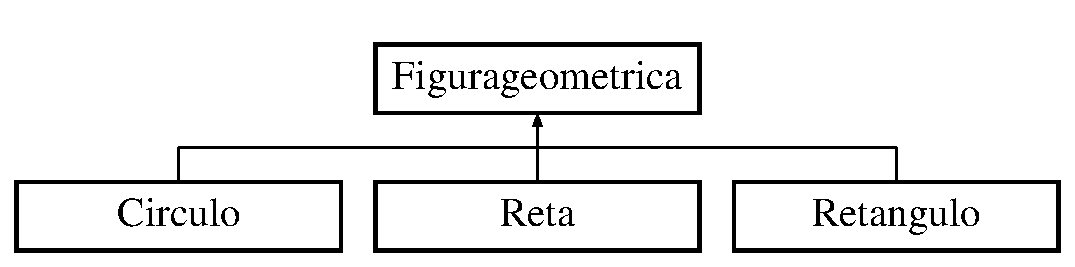
\includegraphics[height=2.000000cm]{class_figurageometrica}
\end{center}
\end{figure}
\subsection*{Public Member Functions}
\begin{DoxyCompactItemize}
\item 
\mbox{\Hypertarget{class_figurageometrica_aaa6a63e714e6ee3e884d17a5151b1ec4}\label{class_figurageometrica_aaa6a63e714e6ee3e884d17a5151b1ec4}} 
\mbox{\hyperlink{class_figurageometrica_aaa6a63e714e6ee3e884d17a5151b1ec4}{Figurageometrica}} ()
\begin{DoxyCompactList}\small\item\em \mbox{\hyperlink{class_figurageometrica}{Figurageometrica}} Construtor padrão da classe figuras geomátricas. \end{DoxyCompactList}\item 
virtual void \mbox{\hyperlink{class_figurageometrica_a68d9aba508879bb7a9ea1fe9d1d4f5f4}{draw}} (\mbox{\hyperlink{class_screen}{Screen}} \&t)=0
\begin{DoxyCompactList}\small\item\em draw Função virtual pura para ser chamada dependendo da figura geométrica \end{DoxyCompactList}\end{DoxyCompactItemize}
\subsection*{Protected Attributes}
\begin{DoxyCompactItemize}
\item 
\mbox{\Hypertarget{class_figurageometrica_a7fe8a9843c286befdf0b96871d6e0a4b}\label{class_figurageometrica_a7fe8a9843c286befdf0b96871d6e0a4b}} 
vector$<$ \mbox{\hyperlink{class_ponto}{Ponto}} $>$ \mbox{\hyperlink{class_figurageometrica_a7fe8a9843c286befdf0b96871d6e0a4b}{p}}
\begin{DoxyCompactList}\small\item\em p Vector de pontos para guardar os pontos importantes das figuras geométricas \end{DoxyCompactList}\end{DoxyCompactItemize}


\subsection{Detailed Description}
The \mbox{\hyperlink{class_figurageometrica}{Figurageometrica}} class Classe para representar figuras geométricas, possui um vetor que guarda vários tipos de figuras geométricas. 

\subsection{Member Function Documentation}
\mbox{\Hypertarget{class_figurageometrica_a68d9aba508879bb7a9ea1fe9d1d4f5f4}\label{class_figurageometrica_a68d9aba508879bb7a9ea1fe9d1d4f5f4}} 
\index{Figurageometrica@{Figurageometrica}!draw@{draw}}
\index{draw@{draw}!Figurageometrica@{Figurageometrica}}
\subsubsection{\texorpdfstring{draw()}{draw()}}
{\footnotesize\ttfamily virtual void Figurageometrica\+::draw (\begin{DoxyParamCaption}\item[{\mbox{\hyperlink{class_screen}{Screen}} \&}]{t }\end{DoxyParamCaption})\hspace{0.3cm}{\ttfamily [pure virtual]}}



draw Função virtual pura para ser chamada dependendo da figura geométrica 


\begin{DoxyParams}{Parameters}
{\em t} & Matriz para desenhar as figuras geométricas \\
\hline
\end{DoxyParams}


Implemented in \mbox{\hyperlink{class_retangulo_ac088dd6d3f4f3d3f80363a868c2e74f1}{Retangulo}}, \mbox{\hyperlink{class_circulo_a593787d6e0618c2eded23e8839e7bea6}{Circulo}}, and \mbox{\hyperlink{class_reta_ac2e9805183cd474b62bffd8b032cd780}{Reta}}.



The documentation for this class was generated from the following files\+:\begin{DoxyCompactItemize}
\item 
figurageometrica.\+h\item 
figurageometrica.\+cpp\end{DoxyCompactItemize}

\hypertarget{class_ponto}{}\section{Ponto Class Reference}
\label{class_ponto}\index{Ponto@{Ponto}}


The \mbox{\hyperlink{class_ponto}{Ponto}} class Classe para representar pontos das figuras geométricas.  




{\ttfamily \#include $<$ponto.\+h$>$}

\subsection*{Public Member Functions}
\begin{DoxyCompactItemize}
\item 
\mbox{\hyperlink{class_ponto_aab845b69e717a88f821eac509ae61d0c}{Ponto}} (int \+\_\+x, int \+\_\+y)
\begin{DoxyCompactList}\small\item\em \mbox{\hyperlink{class_ponto}{Ponto}} Construtor da classe ponto com parâmetros iniciais. \end{DoxyCompactList}\item 
int \mbox{\hyperlink{class_ponto_a46143a67138fec36b9aa71903accee5a}{getx}} ()
\begin{DoxyCompactList}\small\item\em getx Método para retornar o valor da coordenada x \end{DoxyCompactList}\item 
void \mbox{\hyperlink{class_ponto_ab49e43abd7833943dc2caaa6dff012c2}{setx}} (int \+\_\+x)
\begin{DoxyCompactList}\small\item\em setx Método para mudar o valor guardado na variável x \end{DoxyCompactList}\item 
int \mbox{\hyperlink{class_ponto_a383a1698d34a2bc2cc84293e951d0f3b}{gety}} ()
\begin{DoxyCompactList}\small\item\em gety Método para retornar o valor da coordenada y \end{DoxyCompactList}\item 
void \mbox{\hyperlink{class_ponto_a13ea5b12596fc0b8b725115d56404e20}{sety}} (int \+\_\+y)
\begin{DoxyCompactList}\small\item\em sety Método para mudar o valor guardado na variável y \end{DoxyCompactList}\end{DoxyCompactItemize}


\subsection{Detailed Description}
The \mbox{\hyperlink{class_ponto}{Ponto}} class Classe para representar pontos das figuras geométricas. 

\subsection{Constructor \& Destructor Documentation}
\mbox{\Hypertarget{class_ponto_aab845b69e717a88f821eac509ae61d0c}\label{class_ponto_aab845b69e717a88f821eac509ae61d0c}} 
\index{Ponto@{Ponto}!Ponto@{Ponto}}
\index{Ponto@{Ponto}!Ponto@{Ponto}}
\subsubsection{\texorpdfstring{Ponto()}{Ponto()}}
{\footnotesize\ttfamily Ponto\+::\+Ponto (\begin{DoxyParamCaption}\item[{int}]{\+\_\+x,  }\item[{int}]{\+\_\+y }\end{DoxyParamCaption})}



\mbox{\hyperlink{class_ponto}{Ponto}} Construtor da classe ponto com parâmetros iniciais. 


\begin{DoxyParams}{Parameters}
{\em \+\_\+x} & Coordenada x inicial \\
\hline
{\em \+\_\+y} & Coordenada y inicial \\
\hline
\end{DoxyParams}


\subsection{Member Function Documentation}
\mbox{\Hypertarget{class_ponto_a46143a67138fec36b9aa71903accee5a}\label{class_ponto_a46143a67138fec36b9aa71903accee5a}} 
\index{Ponto@{Ponto}!getx@{getx}}
\index{getx@{getx}!Ponto@{Ponto}}
\subsubsection{\texorpdfstring{getx()}{getx()}}
{\footnotesize\ttfamily int Ponto\+::getx (\begin{DoxyParamCaption}{ }\end{DoxyParamCaption})}



getx Método para retornar o valor da coordenada x 

\begin{DoxyReturn}{Returns}
Retorna um int com o valor guardado na coordenada x 
\end{DoxyReturn}
\mbox{\Hypertarget{class_ponto_a383a1698d34a2bc2cc84293e951d0f3b}\label{class_ponto_a383a1698d34a2bc2cc84293e951d0f3b}} 
\index{Ponto@{Ponto}!gety@{gety}}
\index{gety@{gety}!Ponto@{Ponto}}
\subsubsection{\texorpdfstring{gety()}{gety()}}
{\footnotesize\ttfamily int Ponto\+::gety (\begin{DoxyParamCaption}{ }\end{DoxyParamCaption})}



gety Método para retornar o valor da coordenada y 

\begin{DoxyReturn}{Returns}
Retorna um int com o valor guardado na coordenada y 
\end{DoxyReturn}
\mbox{\Hypertarget{class_ponto_ab49e43abd7833943dc2caaa6dff012c2}\label{class_ponto_ab49e43abd7833943dc2caaa6dff012c2}} 
\index{Ponto@{Ponto}!setx@{setx}}
\index{setx@{setx}!Ponto@{Ponto}}
\subsubsection{\texorpdfstring{setx()}{setx()}}
{\footnotesize\ttfamily void Ponto\+::setx (\begin{DoxyParamCaption}\item[{int}]{\+\_\+x }\end{DoxyParamCaption})}



setx Método para mudar o valor guardado na variável x 


\begin{DoxyParams}{Parameters}
{\em \+\_\+x} & Valor que será colocado na variável x \\
\hline
\end{DoxyParams}
\mbox{\Hypertarget{class_ponto_a13ea5b12596fc0b8b725115d56404e20}\label{class_ponto_a13ea5b12596fc0b8b725115d56404e20}} 
\index{Ponto@{Ponto}!sety@{sety}}
\index{sety@{sety}!Ponto@{Ponto}}
\subsubsection{\texorpdfstring{sety()}{sety()}}
{\footnotesize\ttfamily void Ponto\+::sety (\begin{DoxyParamCaption}\item[{int}]{\+\_\+y }\end{DoxyParamCaption})}



sety Método para mudar o valor guardado na variável y 


\begin{DoxyParams}{Parameters}
{\em \+\_\+y} & Valor que será colocado na variável y \\
\hline
\end{DoxyParams}


The documentation for this class was generated from the following files\+:\begin{DoxyCompactItemize}
\item 
\mbox{\hyperlink{ponto_8h}{ponto.\+h}}\item 
\mbox{\hyperlink{ponto_8cpp}{ponto.\+cpp}}\end{DoxyCompactItemize}

\hypertarget{class_reta}{}\section{Reta Class Reference}
\label{class_reta}\index{Reta@{Reta}}


The \mbox{\hyperlink{class_reta}{Reta}} class Classe para representar uma reta.  




{\ttfamily \#include $<$reta.\+h$>$}

Inheritance diagram for Reta\+:\begin{figure}[H]
\begin{center}
\leavevmode
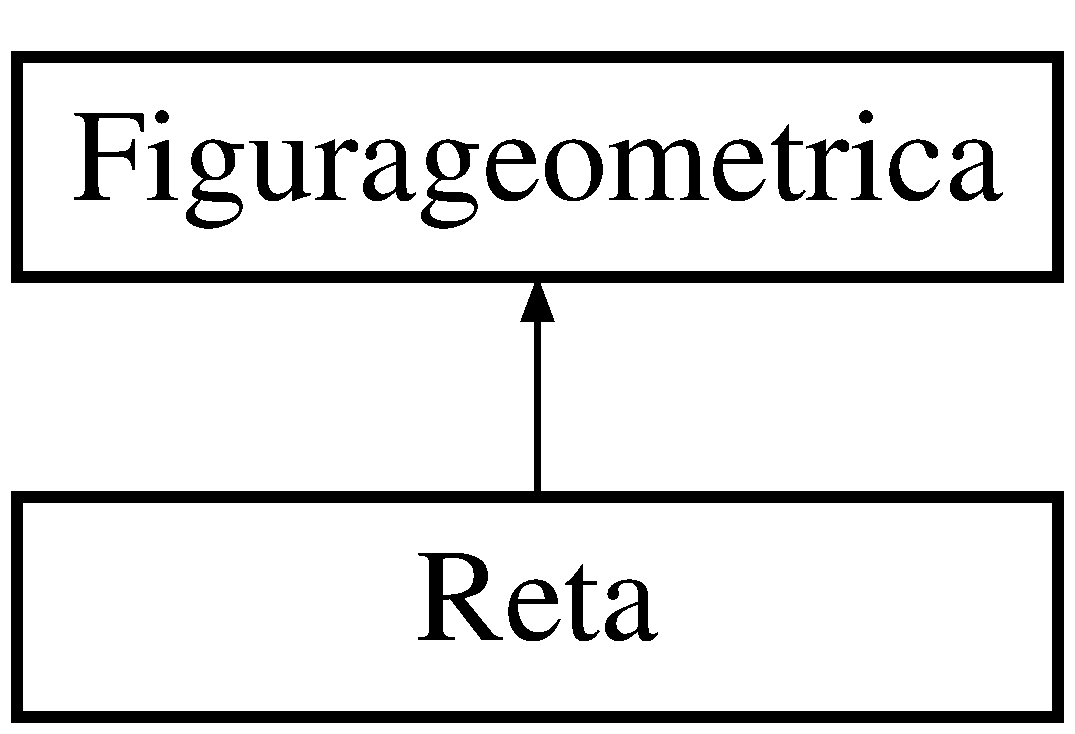
\includegraphics[height=2.000000cm]{class_reta}
\end{center}
\end{figure}
\subsection*{Public Member Functions}
\begin{DoxyCompactItemize}
\item 
\mbox{\hyperlink{class_reta_a79c6845d930a7762d80224e5857fe3da}{Reta}} (\mbox{\hyperlink{class_ponto}{Ponto}} p1, \mbox{\hyperlink{class_ponto}{Ponto}} p2)
\begin{DoxyCompactList}\small\item\em \mbox{\hyperlink{class_reta}{Reta}} Construtor da classe reta que inicia com valores passados por parâmetro. \end{DoxyCompactList}\item 
void \mbox{\hyperlink{class_reta_ac2e9805183cd474b62bffd8b032cd780}{draw}} (\mbox{\hyperlink{class_screen}{Screen}} \&t)
\begin{DoxyCompactList}\small\item\em draw Função virtual para desenhar uma reta quando chamado \end{DoxyCompactList}\end{DoxyCompactItemize}
\subsection*{Additional Inherited Members}


\subsection{Detailed Description}
The \mbox{\hyperlink{class_reta}{Reta}} class Classe para representar uma reta. 

\subsection{Constructor \& Destructor Documentation}
\mbox{\Hypertarget{class_reta_a79c6845d930a7762d80224e5857fe3da}\label{class_reta_a79c6845d930a7762d80224e5857fe3da}} 
\index{Reta@{Reta}!Reta@{Reta}}
\index{Reta@{Reta}!Reta@{Reta}}
\subsubsection{\texorpdfstring{Reta()}{Reta()}}
{\footnotesize\ttfamily Reta\+::\+Reta (\begin{DoxyParamCaption}\item[{\mbox{\hyperlink{class_ponto}{Ponto}}}]{p1,  }\item[{\mbox{\hyperlink{class_ponto}{Ponto}}}]{p2 }\end{DoxyParamCaption})}



\mbox{\hyperlink{class_reta}{Reta}} Construtor da classe reta que inicia com valores passados por parâmetro. 


\begin{DoxyParams}{Parameters}
{\em p1} & \mbox{\hyperlink{class_ponto}{Ponto}} onde começa a reta \\
\hline
{\em p2} & \mbox{\hyperlink{class_ponto}{Ponto}} onde termina a reta \\
\hline
\end{DoxyParams}


\subsection{Member Function Documentation}
\mbox{\Hypertarget{class_reta_ac2e9805183cd474b62bffd8b032cd780}\label{class_reta_ac2e9805183cd474b62bffd8b032cd780}} 
\index{Reta@{Reta}!draw@{draw}}
\index{draw@{draw}!Reta@{Reta}}
\subsubsection{\texorpdfstring{draw()}{draw()}}
{\footnotesize\ttfamily void Reta\+::draw (\begin{DoxyParamCaption}\item[{\mbox{\hyperlink{class_screen}{Screen}} \&}]{t }\end{DoxyParamCaption})\hspace{0.3cm}{\ttfamily [virtual]}}



draw Função virtual para desenhar uma reta quando chamado 


\begin{DoxyParams}{Parameters}
{\em t} & Matriz onde será desenhado a reta \\
\hline
\end{DoxyParams}


Implements \mbox{\hyperlink{class_figurageometrica_a68d9aba508879bb7a9ea1fe9d1d4f5f4}{Figurageometrica}}.



The documentation for this class was generated from the following files\+:\begin{DoxyCompactItemize}
\item 
\mbox{\hyperlink{reta_8h}{reta.\+h}}\item 
\mbox{\hyperlink{reta_8cpp}{reta.\+cpp}}\end{DoxyCompactItemize}

\hypertarget{class_retangulo}{}\section{Retangulo Class Reference}
\label{class_retangulo}\index{Retangulo@{Retangulo}}


The \mbox{\hyperlink{class_retangulo}{Retangulo}} class Classe para representar um retângulo.  




{\ttfamily \#include $<$retangulo.\+h$>$}

Inheritance diagram for Retangulo\+:\begin{figure}[H]
\begin{center}
\leavevmode
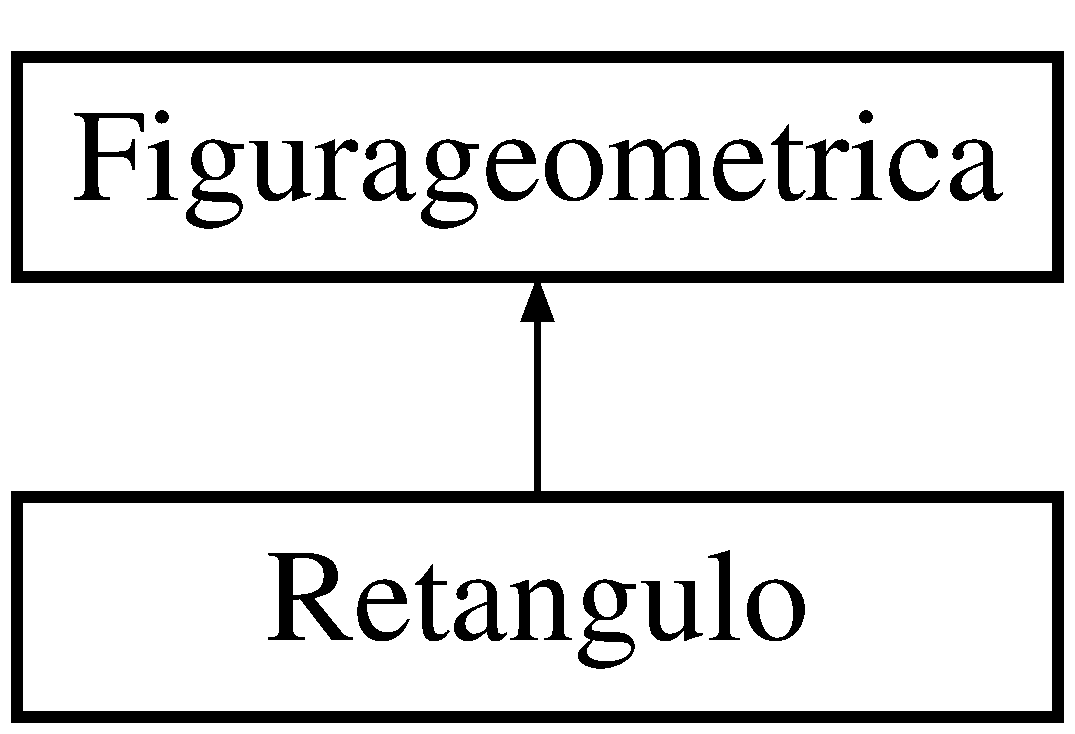
\includegraphics[height=2.000000cm]{class_retangulo}
\end{center}
\end{figure}
\subsection*{Public Member Functions}
\begin{DoxyCompactItemize}
\item 
\mbox{\hyperlink{class_retangulo_a2ffbe31f15ad438225568f3e6d246e62}{Retangulo}} (\mbox{\hyperlink{class_ponto}{Ponto}} \+\_\+p1, int largura, int altura, bool \+\_\+fillmolde)
\begin{DoxyCompactList}\small\item\em \mbox{\hyperlink{class_retangulo}{Retangulo}} Construtuor da classe com valores inicias. \end{DoxyCompactList}\item 
void \mbox{\hyperlink{class_retangulo_a6dec6e7cba5c6de8834b00599ee1e150}{setfillmolde}} (bool \+\_\+fillmolde)
\begin{DoxyCompactList}\small\item\em setfillmolde Método para mudar o valor do molde \end{DoxyCompactList}\item 
void \mbox{\hyperlink{class_retangulo_afaaf315f9be859d0d83bae99baf645cb}{setlargura}} (int \+\_\+largura)
\begin{DoxyCompactList}\small\item\em setlargura Método para mudar o valor da largura \end{DoxyCompactList}\item 
void \mbox{\hyperlink{class_retangulo_aa4c2a5395874545b17c28743a4362a6f}{setaltura}} (int \+\_\+altura)
\begin{DoxyCompactList}\small\item\em setaltura Método para mudar o valor da altura \end{DoxyCompactList}\item 
int \mbox{\hyperlink{class_retangulo_a44414c2c20da988fec6ec12722ae95dc}{getlargura}} ()
\begin{DoxyCompactList}\small\item\em getlargura Método que retorna o valor guardado na variável largura \end{DoxyCompactList}\item 
int \mbox{\hyperlink{class_retangulo_a42d313847d429dda0869873a7b0e47a1}{getaltura}} ()
\begin{DoxyCompactList}\small\item\em getaltura Método que retorna o valor guardado na variável altura \end{DoxyCompactList}\item 
void \mbox{\hyperlink{class_retangulo_ac088dd6d3f4f3d3f80363a868c2e74f1}{draw}} (\mbox{\hyperlink{class_screen}{Screen}} \&t)
\begin{DoxyCompactList}\small\item\em draw Função virtual que irá ser chamada quando desenhar o retangulo \end{DoxyCompactList}\end{DoxyCompactItemize}
\subsection*{Additional Inherited Members}


\subsection{Detailed Description}
The \mbox{\hyperlink{class_retangulo}{Retangulo}} class Classe para representar um retângulo. 

\subsection{Constructor \& Destructor Documentation}
\mbox{\Hypertarget{class_retangulo_a2ffbe31f15ad438225568f3e6d246e62}\label{class_retangulo_a2ffbe31f15ad438225568f3e6d246e62}} 
\index{Retangulo@{Retangulo}!Retangulo@{Retangulo}}
\index{Retangulo@{Retangulo}!Retangulo@{Retangulo}}
\subsubsection{\texorpdfstring{Retangulo()}{Retangulo()}}
{\footnotesize\ttfamily Retangulo\+::\+Retangulo (\begin{DoxyParamCaption}\item[{\mbox{\hyperlink{class_ponto}{Ponto}}}]{\+\_\+p1,  }\item[{int}]{largura,  }\item[{int}]{altura,  }\item[{bool}]{\+\_\+fillmolde }\end{DoxyParamCaption})}



\mbox{\hyperlink{class_retangulo}{Retangulo}} Construtuor da classe com valores inicias. 


\begin{DoxyParams}{Parameters}
{\em \+\_\+p1} & \mbox{\hyperlink{class_ponto}{Ponto}} do canto superior esquerdo do retângulo \\
\hline
{\em largura} & Valor inicial da largura \\
\hline
{\em altura} & Valor inicial da altura \\
\hline
{\em \+\_\+fillmolde} & Valor inicial do molde \\
\hline
\end{DoxyParams}


\subsection{Member Function Documentation}
\mbox{\Hypertarget{class_retangulo_ac088dd6d3f4f3d3f80363a868c2e74f1}\label{class_retangulo_ac088dd6d3f4f3d3f80363a868c2e74f1}} 
\index{Retangulo@{Retangulo}!draw@{draw}}
\index{draw@{draw}!Retangulo@{Retangulo}}
\subsubsection{\texorpdfstring{draw()}{draw()}}
{\footnotesize\ttfamily void Retangulo\+::draw (\begin{DoxyParamCaption}\item[{\mbox{\hyperlink{class_screen}{Screen}} \&}]{t }\end{DoxyParamCaption})\hspace{0.3cm}{\ttfamily [virtual]}}



draw Função virtual que irá ser chamada quando desenhar o retangulo 


\begin{DoxyParams}{Parameters}
{\em t} & Matriz onde será desenhado o retangulo \\
\hline
\end{DoxyParams}


Implements \mbox{\hyperlink{class_figurageometrica_a68d9aba508879bb7a9ea1fe9d1d4f5f4}{Figurageometrica}}.

\mbox{\Hypertarget{class_retangulo_a42d313847d429dda0869873a7b0e47a1}\label{class_retangulo_a42d313847d429dda0869873a7b0e47a1}} 
\index{Retangulo@{Retangulo}!getaltura@{getaltura}}
\index{getaltura@{getaltura}!Retangulo@{Retangulo}}
\subsubsection{\texorpdfstring{getaltura()}{getaltura()}}
{\footnotesize\ttfamily int Retangulo\+::getaltura (\begin{DoxyParamCaption}{ }\end{DoxyParamCaption})}



getaltura Método que retorna o valor guardado na variável altura 

\begin{DoxyReturn}{Returns}
Retorna um inteiro com o valor da altura do retangulo 
\end{DoxyReturn}
\mbox{\Hypertarget{class_retangulo_a44414c2c20da988fec6ec12722ae95dc}\label{class_retangulo_a44414c2c20da988fec6ec12722ae95dc}} 
\index{Retangulo@{Retangulo}!getlargura@{getlargura}}
\index{getlargura@{getlargura}!Retangulo@{Retangulo}}
\subsubsection{\texorpdfstring{getlargura()}{getlargura()}}
{\footnotesize\ttfamily int Retangulo\+::getlargura (\begin{DoxyParamCaption}{ }\end{DoxyParamCaption})}



getlargura Método que retorna o valor guardado na variável largura 

\begin{DoxyReturn}{Returns}
Retorna um inteiro com o valor da altura do retangulo 
\end{DoxyReturn}
\mbox{\Hypertarget{class_retangulo_aa4c2a5395874545b17c28743a4362a6f}\label{class_retangulo_aa4c2a5395874545b17c28743a4362a6f}} 
\index{Retangulo@{Retangulo}!setaltura@{setaltura}}
\index{setaltura@{setaltura}!Retangulo@{Retangulo}}
\subsubsection{\texorpdfstring{setaltura()}{setaltura()}}
{\footnotesize\ttfamily void Retangulo\+::setaltura (\begin{DoxyParamCaption}\item[{int}]{\+\_\+altura }\end{DoxyParamCaption})}



setaltura Método para mudar o valor da altura 


\begin{DoxyParams}{Parameters}
{\em \+\_\+altura} & Valor que irá ser guardado na variável altura \\
\hline
\end{DoxyParams}
\mbox{\Hypertarget{class_retangulo_a6dec6e7cba5c6de8834b00599ee1e150}\label{class_retangulo_a6dec6e7cba5c6de8834b00599ee1e150}} 
\index{Retangulo@{Retangulo}!setfillmolde@{setfillmolde}}
\index{setfillmolde@{setfillmolde}!Retangulo@{Retangulo}}
\subsubsection{\texorpdfstring{setfillmolde()}{setfillmolde()}}
{\footnotesize\ttfamily void Retangulo\+::setfillmolde (\begin{DoxyParamCaption}\item[{bool}]{\+\_\+fillmolde }\end{DoxyParamCaption})}



setfillmolde Método para mudar o valor do molde 


\begin{DoxyParams}{Parameters}
{\em \+\_\+fillmolde} & Parâmetro que irá trocar o valor do molde \\
\hline
\end{DoxyParams}
\mbox{\Hypertarget{class_retangulo_afaaf315f9be859d0d83bae99baf645cb}\label{class_retangulo_afaaf315f9be859d0d83bae99baf645cb}} 
\index{Retangulo@{Retangulo}!setlargura@{setlargura}}
\index{setlargura@{setlargura}!Retangulo@{Retangulo}}
\subsubsection{\texorpdfstring{setlargura()}{setlargura()}}
{\footnotesize\ttfamily void Retangulo\+::setlargura (\begin{DoxyParamCaption}\item[{int}]{\+\_\+largura }\end{DoxyParamCaption})}



setlargura Método para mudar o valor da largura 


\begin{DoxyParams}{Parameters}
{\em \+\_\+largura} & Valor que irá ser guardado na variável largura \\
\hline
\end{DoxyParams}


The documentation for this class was generated from the following files\+:\begin{DoxyCompactItemize}
\item 
retangulo.\+h\item 
retangulo.\+cpp\end{DoxyCompactItemize}

\hypertarget{class_screen}{}\section{Screen Class Reference}
\label{class_screen}\index{Screen@{Screen}}


The \mbox{\hyperlink{class_screen}{Screen}} class Classe para representar uma tela onde será desenhada as figuras geométrica.  




{\ttfamily \#include $<$screen.\+h$>$}

\subsection*{Public Member Functions}
\begin{DoxyCompactItemize}
\item 
\mbox{\Hypertarget{class_screen_ae7576476fc6e6a6eaa66389fdc41fe72}\label{class_screen_ae7576476fc6e6a6eaa66389fdc41fe72}} 
\mbox{\hyperlink{class_screen_ae7576476fc6e6a6eaa66389fdc41fe72}{Screen}} ()
\begin{DoxyCompactList}\small\item\em \mbox{\hyperlink{class_screen}{Screen}} Construtor padrão da classe. \end{DoxyCompactList}\item 
void \mbox{\hyperlink{class_screen_ac4d187efda643cfc9127230d6363c721}{setnlim}} (int \+\_\+nlin)
\begin{DoxyCompactList}\small\item\em setnlim Método para mudar o valor do número de linhas da tela \end{DoxyCompactList}\item 
void \mbox{\hyperlink{class_screen_a07a26006fcf8b8169af511f1eff03a04}{setncol}} (int \+\_\+ncol)
\begin{DoxyCompactList}\small\item\em setncol Método para mudar o valor do número de colunas da tela \end{DoxyCompactList}\item 
void \mbox{\hyperlink{class_screen_a3570e45d7dbc261cc4da471259a66d7a}{alocamat}} (int \+\_\+nlin, int \+\_\+ncol)
\begin{DoxyCompactList}\small\item\em alocamat Método que aloca o tamanho da tela \end{DoxyCompactList}\item 
int \mbox{\hyperlink{class_screen_ac247e58a4575bbafa46b9f9d24841538}{getnlin}} ()
\begin{DoxyCompactList}\small\item\em getnlin Método que retorna a quantidade de linhas da tela \end{DoxyCompactList}\item 
int \mbox{\hyperlink{class_screen_abaae93e39587a865d4ac1f7fa1a501c2}{getncol}} ()
\begin{DoxyCompactList}\small\item\em getncol Método que retorna a quantidade de colunas da tela \end{DoxyCompactList}\item 
void \mbox{\hyperlink{class_screen_ae6bea81c57a22d226507c3c26fa95ee0}{set\+Pixel}} (int x, int y)
\begin{DoxyCompactList}\small\item\em set\+Pixel Método que muda o \char`\"{}pixel\char`\"{} com o valor do \textquotesingle{}brush\textquotesingle{}, representado como uma coordenada de uma matriz \end{DoxyCompactList}\item 
\mbox{\Hypertarget{class_screen_a35e74266b2a04e37b354ceff7a5f1031}\label{class_screen_a35e74266b2a04e37b354ceff7a5f1031}} 
void \mbox{\hyperlink{class_screen_a35e74266b2a04e37b354ceff7a5f1031}{clear}} ()
\begin{DoxyCompactList}\small\item\em clear Método que limpa a tela, muda todos o valores atuais da tela para o valor inicial \end{DoxyCompactList}\item 
void \mbox{\hyperlink{class_screen_aebc4eb6cb5acf15a0f04c1494622ab23}{set\+Brush}} (char \+\_\+brush)
\begin{DoxyCompactList}\small\item\em set\+Brush Método que muda o caractere com qual queremos desenhar as figuras \end{DoxyCompactList}\item 
\mbox{\Hypertarget{class_screen_ad0d7ac072702d42e6a920a806fbc79e2}\label{class_screen_ad0d7ac072702d42e6a920a806fbc79e2}} 
void \mbox{\hyperlink{class_screen_ad0d7ac072702d42e6a920a806fbc79e2}{salvafigura}} ()
\begin{DoxyCompactList}\small\item\em salvafigura Método que salva a tela atual em um arquivo \end{DoxyCompactList}\end{DoxyCompactItemize}
\subsection*{Friends}
\begin{DoxyCompactItemize}
\item 
ostream \& \mbox{\hyperlink{class_screen_aab6a2880746bfe1b7964817cc8f0989e}{operator$<$$<$}} (ostream \&os, \mbox{\hyperlink{class_screen}{Screen}} \&t)
\begin{DoxyCompactList}\small\item\em operator $<$$<$ Operador $<$$<$ para imprimir a tela em forma de matriz \end{DoxyCompactList}\item 
void \mbox{\hyperlink{class_screen_adbcadcf484d39b99a5653dbb66ebc373}{desenhareta}} (int x1, int y1, int x2, int y2, \mbox{\hyperlink{class_screen}{Screen}} \&t)
\begin{DoxyCompactList}\small\item\em desenhareta Método que altera as coordenadas da tela com o \char`\"{}pincel\char`\"{} usando o algoritmo de Bresenham para desenhar retas \end{DoxyCompactList}\item 
void \mbox{\hyperlink{class_screen_a7528dc26ec23f8212f5a0748a09884f1}{desenharetangulo}} (\mbox{\hyperlink{class_ponto}{Ponto}} p, int largura, int altura, \mbox{\hyperlink{class_screen}{Screen}} \&t, bool \+\_\+fillmolde)
\begin{DoxyCompactList}\small\item\em desenharetangulo Método que altera as coordenadas da tela com o \char`\"{}pincel\char`\"{} \end{DoxyCompactList}\item 
void \mbox{\hyperlink{class_screen_adcbc719000bbfb8a9354328c32147ff2}{desenhacirculo}} (int \+\_\+x, int \+\_\+y, int radius, \mbox{\hyperlink{class_screen}{Screen}} \&t, bool \+\_\+fillmolde)
\begin{DoxyCompactList}\small\item\em desenhacirculo Método que altera as coordenadas da tela com o \char`\"{}pincel\char`\"{} usando o algoritmo de Bresenham para desenhar circulos \end{DoxyCompactList}\end{DoxyCompactItemize}


\subsection{Detailed Description}
The \mbox{\hyperlink{class_screen}{Screen}} class Classe para representar uma tela onde será desenhada as figuras geométrica. 

\subsection{Member Function Documentation}
\mbox{\Hypertarget{class_screen_a3570e45d7dbc261cc4da471259a66d7a}\label{class_screen_a3570e45d7dbc261cc4da471259a66d7a}} 
\index{Screen@{Screen}!alocamat@{alocamat}}
\index{alocamat@{alocamat}!Screen@{Screen}}
\subsubsection{\texorpdfstring{alocamat()}{alocamat()}}
{\footnotesize\ttfamily void Screen\+::alocamat (\begin{DoxyParamCaption}\item[{int}]{\+\_\+nlin,  }\item[{int}]{\+\_\+ncol }\end{DoxyParamCaption})}



alocamat Método que aloca o tamanho da tela 


\begin{DoxyParams}{Parameters}
{\em \+\_\+nlin} & Número de linhas que a tela terá \\
\hline
{\em \+\_\+ncol} & Número de colunas que a tela terá \\
\hline
\end{DoxyParams}
\mbox{\Hypertarget{class_screen_abaae93e39587a865d4ac1f7fa1a501c2}\label{class_screen_abaae93e39587a865d4ac1f7fa1a501c2}} 
\index{Screen@{Screen}!getncol@{getncol}}
\index{getncol@{getncol}!Screen@{Screen}}
\subsubsection{\texorpdfstring{getncol()}{getncol()}}
{\footnotesize\ttfamily int Screen\+::getncol (\begin{DoxyParamCaption}{ }\end{DoxyParamCaption})}



getncol Método que retorna a quantidade de colunas da tela 

\begin{DoxyReturn}{Returns}
Retorna um inteiro que é o número de linhas da tela 
\end{DoxyReturn}
\mbox{\Hypertarget{class_screen_ac247e58a4575bbafa46b9f9d24841538}\label{class_screen_ac247e58a4575bbafa46b9f9d24841538}} 
\index{Screen@{Screen}!getnlin@{getnlin}}
\index{getnlin@{getnlin}!Screen@{Screen}}
\subsubsection{\texorpdfstring{getnlin()}{getnlin()}}
{\footnotesize\ttfamily int Screen\+::getnlin (\begin{DoxyParamCaption}{ }\end{DoxyParamCaption})}



getnlin Método que retorna a quantidade de linhas da tela 

\begin{DoxyReturn}{Returns}
Retorna um inteiro que é o número de linhas da tela 
\end{DoxyReturn}
\mbox{\Hypertarget{class_screen_aebc4eb6cb5acf15a0f04c1494622ab23}\label{class_screen_aebc4eb6cb5acf15a0f04c1494622ab23}} 
\index{Screen@{Screen}!set\+Brush@{set\+Brush}}
\index{set\+Brush@{set\+Brush}!Screen@{Screen}}
\subsubsection{\texorpdfstring{set\+Brush()}{setBrush()}}
{\footnotesize\ttfamily void Screen\+::set\+Brush (\begin{DoxyParamCaption}\item[{char}]{\+\_\+brush }\end{DoxyParamCaption})}



set\+Brush Método que muda o caractere com qual queremos desenhar as figuras 


\begin{DoxyParams}{Parameters}
{\em \+\_\+brush} & Caractere que troca o pincel \\
\hline
\end{DoxyParams}
\mbox{\Hypertarget{class_screen_a07a26006fcf8b8169af511f1eff03a04}\label{class_screen_a07a26006fcf8b8169af511f1eff03a04}} 
\index{Screen@{Screen}!setncol@{setncol}}
\index{setncol@{setncol}!Screen@{Screen}}
\subsubsection{\texorpdfstring{setncol()}{setncol()}}
{\footnotesize\ttfamily void Screen\+::setncol (\begin{DoxyParamCaption}\item[{int}]{\+\_\+ncol }\end{DoxyParamCaption})}



setncol Método para mudar o valor do número de colunas da tela 


\begin{DoxyParams}{Parameters}
{\em \+\_\+ncol} & Valor que será guardado na qte de colunas da tela \\
\hline
\end{DoxyParams}
\mbox{\Hypertarget{class_screen_ac4d187efda643cfc9127230d6363c721}\label{class_screen_ac4d187efda643cfc9127230d6363c721}} 
\index{Screen@{Screen}!setnlim@{setnlim}}
\index{setnlim@{setnlim}!Screen@{Screen}}
\subsubsection{\texorpdfstring{setnlim()}{setnlim()}}
{\footnotesize\ttfamily void Screen\+::setnlim (\begin{DoxyParamCaption}\item[{int}]{\+\_\+nlin }\end{DoxyParamCaption})}



setnlim Método para mudar o valor do número de linhas da tela 


\begin{DoxyParams}{Parameters}
{\em \+\_\+nlin} & valor que será guardado na qte de linhas da tela \\
\hline
\end{DoxyParams}
\mbox{\Hypertarget{class_screen_ae6bea81c57a22d226507c3c26fa95ee0}\label{class_screen_ae6bea81c57a22d226507c3c26fa95ee0}} 
\index{Screen@{Screen}!set\+Pixel@{set\+Pixel}}
\index{set\+Pixel@{set\+Pixel}!Screen@{Screen}}
\subsubsection{\texorpdfstring{set\+Pixel()}{setPixel()}}
{\footnotesize\ttfamily void Screen\+::set\+Pixel (\begin{DoxyParamCaption}\item[{int}]{x,  }\item[{int}]{y }\end{DoxyParamCaption})}



set\+Pixel Método que muda o \char`\"{}pixel\char`\"{} com o valor do \textquotesingle{}brush\textquotesingle{}, representado como uma coordenada de uma matriz 


\begin{DoxyParams}{Parameters}
{\em x} & Coordenada x do pixel que será mudado \\
\hline
{\em y} & Coordenada y do pixel que será mudado \\
\hline
\end{DoxyParams}


\subsection{Friends And Related Function Documentation}
\mbox{\Hypertarget{class_screen_adcbc719000bbfb8a9354328c32147ff2}\label{class_screen_adcbc719000bbfb8a9354328c32147ff2}} 
\index{Screen@{Screen}!desenhacirculo@{desenhacirculo}}
\index{desenhacirculo@{desenhacirculo}!Screen@{Screen}}
\subsubsection{\texorpdfstring{desenhacirculo}{desenhacirculo}}
{\footnotesize\ttfamily void desenhacirculo (\begin{DoxyParamCaption}\item[{int}]{\+\_\+x,  }\item[{int}]{\+\_\+y,  }\item[{int}]{radius,  }\item[{\mbox{\hyperlink{class_screen}{Screen}} \&}]{t,  }\item[{bool}]{\+\_\+fillmolde }\end{DoxyParamCaption})\hspace{0.3cm}{\ttfamily [friend]}}



desenhacirculo Método que altera as coordenadas da tela com o \char`\"{}pincel\char`\"{} usando o algoritmo de Bresenham para desenhar circulos 


\begin{DoxyParams}{Parameters}
{\em \+\_\+x} & Coordenada x do centro do circulo \\
\hline
{\em \+\_\+y} & Coordenada y do centro do circulo \\
\hline
{\em radius} & Valor do raio da circunferência \\
\hline
{\em t} & Tela onde estão sendo desenhadas as figuras \\
\hline
{\em \+\_\+fillmolde} & Variável que indica o molde \\
\hline
\end{DoxyParams}
\mbox{\Hypertarget{class_screen_adbcadcf484d39b99a5653dbb66ebc373}\label{class_screen_adbcadcf484d39b99a5653dbb66ebc373}} 
\index{Screen@{Screen}!desenhareta@{desenhareta}}
\index{desenhareta@{desenhareta}!Screen@{Screen}}
\subsubsection{\texorpdfstring{desenhareta}{desenhareta}}
{\footnotesize\ttfamily void desenhareta (\begin{DoxyParamCaption}\item[{int}]{x1,  }\item[{int}]{y1,  }\item[{int}]{x2,  }\item[{int}]{y2,  }\item[{\mbox{\hyperlink{class_screen}{Screen}} \&}]{t }\end{DoxyParamCaption})\hspace{0.3cm}{\ttfamily [friend]}}



desenhareta Método que altera as coordenadas da tela com o \char`\"{}pincel\char`\"{} usando o algoritmo de Bresenham para desenhar retas 


\begin{DoxyParams}{Parameters}
{\em x1} & Coordenada x do ponto inicial \\
\hline
{\em y1} & Coordenada y do ponto inicial \\
\hline
{\em x2} & Coordenada x do ponto final \\
\hline
{\em y2} & Coordenada y do ponto final \\
\hline
{\em t} & Tela em que as figuras estão sendo desenhadas \\
\hline
\end{DoxyParams}
\mbox{\Hypertarget{class_screen_a7528dc26ec23f8212f5a0748a09884f1}\label{class_screen_a7528dc26ec23f8212f5a0748a09884f1}} 
\index{Screen@{Screen}!desenharetangulo@{desenharetangulo}}
\index{desenharetangulo@{desenharetangulo}!Screen@{Screen}}
\subsubsection{\texorpdfstring{desenharetangulo}{desenharetangulo}}
{\footnotesize\ttfamily void desenharetangulo (\begin{DoxyParamCaption}\item[{\mbox{\hyperlink{class_ponto}{Ponto}}}]{p,  }\item[{int}]{largura,  }\item[{int}]{altura,  }\item[{\mbox{\hyperlink{class_screen}{Screen}} \&}]{t,  }\item[{bool}]{\+\_\+fillmolde }\end{DoxyParamCaption})\hspace{0.3cm}{\ttfamily [friend]}}



desenharetangulo Método que altera as coordenadas da tela com o \char`\"{}pincel\char`\"{} 


\begin{DoxyParams}{Parameters}
{\em p} & \mbox{\hyperlink{class_ponto}{Ponto}} do canto superior esquerdo \\
\hline
{\em largura} & Largura do retangulo \\
\hline
{\em altura} & Altura do retangulo \\
\hline
{\em t} & Tela onde está sendo desenhado as figuras \\
\hline
{\em \+\_\+fillmolde} & Variável que indica o molde \\
\hline
\end{DoxyParams}
\mbox{\Hypertarget{class_screen_aab6a2880746bfe1b7964817cc8f0989e}\label{class_screen_aab6a2880746bfe1b7964817cc8f0989e}} 
\index{Screen@{Screen}!operator$<$$<$@{operator$<$$<$}}
\index{operator$<$$<$@{operator$<$$<$}!Screen@{Screen}}
\subsubsection{\texorpdfstring{operator$<$$<$}{operator<<}}
{\footnotesize\ttfamily ostream\& operator$<$$<$ (\begin{DoxyParamCaption}\item[{ostream \&}]{os,  }\item[{\mbox{\hyperlink{class_screen}{Screen}} \&}]{t }\end{DoxyParamCaption})\hspace{0.3cm}{\ttfamily [friend]}}



operator $<$$<$ Operador $<$$<$ para imprimir a tela em forma de matriz 


\begin{DoxyParams}{Parameters}
{\em os} & Objeto do tipo ostream que é um fluxo de saída \\
\hline
{\em t} & Tela onde os desenhos foram escritos \\
\hline
\end{DoxyParams}
\begin{DoxyReturn}{Returns}
Retorna um objeto do tipo ostream que é um fluxo de saída 
\end{DoxyReturn}


The documentation for this class was generated from the following files\+:\begin{DoxyCompactItemize}
\item 
screen.\+h\item 
screen.\+cpp\end{DoxyCompactItemize}

\chapter{File Documentation}
\hypertarget{circulo_8cpp}{}\section{circulo.\+cpp File Reference}
\label{circulo_8cpp}\index{circulo.\+cpp@{circulo.\+cpp}}
{\ttfamily \#include \char`\"{}circulo.\+h\char`\"{}}\newline
{\ttfamily \#include $<$iostream$>$}\newline

\hypertarget{circulo_8h}{}\section{circulo.\+h File Reference}
\label{circulo_8h}\index{circulo.\+h@{circulo.\+h}}
{\ttfamily \#include \char`\"{}figurageometrica.\+h\char`\"{}}\newline
\subsection*{Classes}
\begin{DoxyCompactItemize}
\item 
class \mbox{\hyperlink{class_circulo}{Circulo}}
\begin{DoxyCompactList}\small\item\em The \mbox{\hyperlink{class_circulo}{Circulo}} class Classe para representar uma circunferência ou disco. \end{DoxyCompactList}\end{DoxyCompactItemize}

\hypertarget{figurageometrica_8cpp}{}\section{figurageometrica.\+cpp File Reference}
\label{figurageometrica_8cpp}\index{figurageometrica.\+cpp@{figurageometrica.\+cpp}}
{\ttfamily \#include \char`\"{}figurageometrica.\+h\char`\"{}}\newline

\hypertarget{figurageometrica_8h}{}\section{figurageometrica.\+h File Reference}
\label{figurageometrica_8h}\index{figurageometrica.\+h@{figurageometrica.\+h}}
{\ttfamily \#include \char`\"{}screen.\+h\char`\"{}}\newline
{\ttfamily \#include \char`\"{}ponto.\+h\char`\"{}}\newline
{\ttfamily \#include $<$vector$>$}\newline
\subsection*{Classes}
\begin{DoxyCompactItemize}
\item 
class \mbox{\hyperlink{class_figurageometrica}{Figurageometrica}}
\begin{DoxyCompactList}\small\item\em The \mbox{\hyperlink{class_figurageometrica}{Figurageometrica}} class Classe para representar figuras geométricas, possui um vetor que guarda vários tipos de figuras geométricas. \end{DoxyCompactList}\end{DoxyCompactItemize}

\hypertarget{main_8cpp}{}\section{main.\+cpp File Reference}
\label{main_8cpp}\index{main.\+cpp@{main.\+cpp}}
{\ttfamily \#include $<$iostream$>$}\newline
{\ttfamily \#include $<$vector$>$}\newline
{\ttfamily \#include \char`\"{}figurageometrica.\+h\char`\"{}}\newline
{\ttfamily \#include \char`\"{}reta.\+h\char`\"{}}\newline
{\ttfamily \#include \char`\"{}retangulo.\+h\char`\"{}}\newline
{\ttfamily \#include \char`\"{}circulo.\+h\char`\"{}}\newline
{\ttfamily \#include \char`\"{}ponto.\+h\char`\"{}}\newline
{\ttfamily \#include \char`\"{}screen.\+h\char`\"{}}\newline
{\ttfamily \#include $<$fstream$>$}\newline
\subsection*{Functions}
\begin{DoxyCompactItemize}
\item 
int \mbox{\hyperlink{main_8cpp_ae66f6b31b5ad750f1fe042a706a4e3d4}{main}} ()
\end{DoxyCompactItemize}


\subsection{Function Documentation}
\mbox{\Hypertarget{main_8cpp_ae66f6b31b5ad750f1fe042a706a4e3d4}\label{main_8cpp_ae66f6b31b5ad750f1fe042a706a4e3d4}} 
\index{main.\+cpp@{main.\+cpp}!main@{main}}
\index{main@{main}!main.\+cpp@{main.\+cpp}}
\subsubsection{\texorpdfstring{main()}{main()}}
{\footnotesize\ttfamily int main (\begin{DoxyParamCaption}{ }\end{DoxyParamCaption})}


\hypertarget{ponto_8cpp}{}\section{ponto.\+cpp File Reference}
\label{ponto_8cpp}\index{ponto.\+cpp@{ponto.\+cpp}}
{\ttfamily \#include \char`\"{}ponto.\+h\char`\"{}}\newline

\hypertarget{ponto_8h}{}\section{ponto.\+h File Reference}
\label{ponto_8h}\index{ponto.\+h@{ponto.\+h}}
\subsection*{Classes}
\begin{DoxyCompactItemize}
\item 
class \mbox{\hyperlink{class_ponto}{Ponto}}
\begin{DoxyCompactList}\small\item\em The \mbox{\hyperlink{class_ponto}{Ponto}} class Classe para representar pontos das figuras geométricas. \end{DoxyCompactList}\end{DoxyCompactItemize}

\hypertarget{reta_8cpp}{}\section{reta.\+cpp File Reference}
\label{reta_8cpp}\index{reta.\+cpp@{reta.\+cpp}}
{\ttfamily \#include \char`\"{}reta.\+h\char`\"{}}\newline
{\ttfamily \#include $<$iostream$>$}\newline
{\ttfamily \#include $<$vector$>$}\newline
\subsection*{Functions}
\begin{DoxyCompactItemize}
\item 
int \mbox{\hyperlink{reta_8cpp_a65d66874fc18bd5559dd6b346d58f530}{Sinal}} (int x)
\end{DoxyCompactItemize}


\subsection{Function Documentation}
\mbox{\Hypertarget{reta_8cpp_a65d66874fc18bd5559dd6b346d58f530}\label{reta_8cpp_a65d66874fc18bd5559dd6b346d58f530}} 
\index{reta.\+cpp@{reta.\+cpp}!Sinal@{Sinal}}
\index{Sinal@{Sinal}!reta.\+cpp@{reta.\+cpp}}
\subsubsection{\texorpdfstring{Sinal()}{Sinal()}}
{\footnotesize\ttfamily int Sinal (\begin{DoxyParamCaption}\item[{int}]{x }\end{DoxyParamCaption})}


\hypertarget{reta_8h}{}\section{reta.\+h File Reference}
\label{reta_8h}\index{reta.\+h@{reta.\+h}}
{\ttfamily \#include \char`\"{}figurageometrica.\+h\char`\"{}}\newline
\subsection*{Classes}
\begin{DoxyCompactItemize}
\item 
class \mbox{\hyperlink{class_reta}{Reta}}
\begin{DoxyCompactList}\small\item\em The \mbox{\hyperlink{class_reta}{Reta}} class Classe para representar uma reta. \end{DoxyCompactList}\end{DoxyCompactItemize}

\hypertarget{retangulo_8cpp}{}\section{retangulo.\+cpp File Reference}
\label{retangulo_8cpp}\index{retangulo.\+cpp@{retangulo.\+cpp}}
{\ttfamily \#include \char`\"{}retangulo.\+h\char`\"{}}\newline
{\ttfamily \#include $<$iostream$>$}\newline

\hypertarget{retangulo_8h}{}\section{retangulo.\+h File Reference}
\label{retangulo_8h}\index{retangulo.\+h@{retangulo.\+h}}
{\ttfamily \#include \char`\"{}figurageometrica.\+h\char`\"{}}\newline
\subsection*{Classes}
\begin{DoxyCompactItemize}
\item 
class \mbox{\hyperlink{class_retangulo}{Retangulo}}
\begin{DoxyCompactList}\small\item\em The \mbox{\hyperlink{class_retangulo}{Retangulo}} class Classe para representar um retângulo. \end{DoxyCompactList}\end{DoxyCompactItemize}

\hypertarget{screen_8cpp}{}\section{screen.\+cpp File Reference}
\label{screen_8cpp}\index{screen.\+cpp@{screen.\+cpp}}
{\ttfamily \#include \char`\"{}screen.\+h\char`\"{}}\newline
{\ttfamily \#include $<$string$>$}\newline
{\ttfamily \#include $<$iostream$>$}\newline
{\ttfamily \#include $<$fstream$>$}\newline
\subsection*{Functions}
\begin{DoxyCompactItemize}
\item 
ostream \& \mbox{\hyperlink{screen_8cpp_aab6a2880746bfe1b7964817cc8f0989e}{operator$<$$<$}} (ostream \&os, \mbox{\hyperlink{class_screen}{Screen}} \&t)
\item 
void \mbox{\hyperlink{screen_8cpp_adcbc719000bbfb8a9354328c32147ff2}{desenhacirculo}} (int \+\_\+x, int \+\_\+y, int radius, \mbox{\hyperlink{class_screen}{Screen}} \&t, bool \+\_\+fillmolde)
\end{DoxyCompactItemize}


\subsection{Function Documentation}
\mbox{\Hypertarget{screen_8cpp_adcbc719000bbfb8a9354328c32147ff2}\label{screen_8cpp_adcbc719000bbfb8a9354328c32147ff2}} 
\index{screen.\+cpp@{screen.\+cpp}!desenhacirculo@{desenhacirculo}}
\index{desenhacirculo@{desenhacirculo}!screen.\+cpp@{screen.\+cpp}}
\subsubsection{\texorpdfstring{desenhacirculo()}{desenhacirculo()}}
{\footnotesize\ttfamily void desenhacirculo (\begin{DoxyParamCaption}\item[{int}]{\+\_\+x,  }\item[{int}]{\+\_\+y,  }\item[{int}]{radius,  }\item[{\mbox{\hyperlink{class_screen}{Screen}} \&}]{t,  }\item[{bool}]{\+\_\+fillmolde }\end{DoxyParamCaption})}

\mbox{\Hypertarget{screen_8cpp_aab6a2880746bfe1b7964817cc8f0989e}\label{screen_8cpp_aab6a2880746bfe1b7964817cc8f0989e}} 
\index{screen.\+cpp@{screen.\+cpp}!operator$<$$<$@{operator$<$$<$}}
\index{operator$<$$<$@{operator$<$$<$}!screen.\+cpp@{screen.\+cpp}}
\subsubsection{\texorpdfstring{operator$<$$<$()}{operator<<()}}
{\footnotesize\ttfamily ostream\& operator$<$$<$ (\begin{DoxyParamCaption}\item[{ostream \&}]{os,  }\item[{\mbox{\hyperlink{class_screen}{Screen}} \&}]{t }\end{DoxyParamCaption})}


\begin{DoxyParams}{Parameters}
{\em os} & Objeto do tipo ostream que é um fluxo de saída \\
\hline
{\em t} & Tela onde os desenhos foram escritos \\
\hline
\end{DoxyParams}
\begin{DoxyReturn}{Returns}
Retorna um objeto do tipo ostream que é um fluxo de saída 
\end{DoxyReturn}

\hypertarget{screen_8h}{}\section{screen.\+h File Reference}
\label{screen_8h}\index{screen.\+h@{screen.\+h}}
{\ttfamily \#include $<$vector$>$}\newline
{\ttfamily \#include $<$ostream$>$}\newline
{\ttfamily \#include \char`\"{}ponto.\+h\char`\"{}}\newline
\subsection*{Classes}
\begin{DoxyCompactItemize}
\item 
class \mbox{\hyperlink{class_screen}{Screen}}
\begin{DoxyCompactList}\small\item\em The \mbox{\hyperlink{class_screen}{Screen}} class Classe para representar uma tela onde será desenhada as figuras geométrica. \end{DoxyCompactList}\end{DoxyCompactItemize}

%--- End generated contents ---

% Index
\backmatter
\newpage
\phantomsection
\clearemptydoublepage
\addcontentsline{toc}{chapter}{Index}
\printindex

\end{document}
